\section{Concept Drift Sources}
\vspace{-3mm}
\begin{figure}[H]
    \centering
    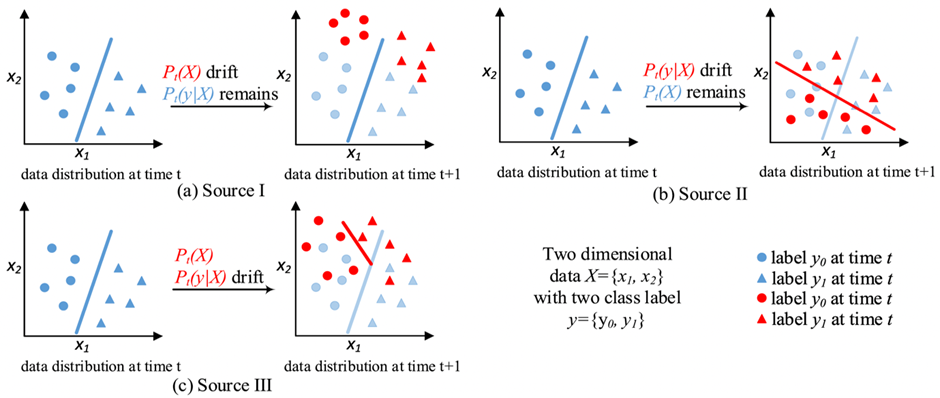
\includegraphics[width=1.0\textwidth]{2_Background/figures/concept_drift_sources.png}
    \caption{Sources of Concept Drift \cite{8496795}. \\ \textcolor{gray}{\fontsize{10}{0}\selectfont DOI: 10.1109/TKDE.2018.2876857}}
    \label{fig:concept-drift-sources}
\end{figure}
\vspace{-6mm}
\label{sec:background_concept_drift_sources}
Concept drift, as illustrated in Fig. \ref{fig:concept-drift-sources}, occurs in three distinct scenarios. First, (a) depicts a shift in data distribution, indicating changes in the underlying patterns and characteristics of incoming data, challenging the model's ability to adapt to new trends \cite{lu2016concept, gama2014survey, losing2016knn, storkey2008training}. Second, (b) shows a change in function output, requiring adjustments in the class delimiter's position as the relationship between input features and output classes evolves. Lastly, (c) represents a dual shift in both data distribution and function output, a more complex form of concept drift that requires the model to adapt to simultaneous changes in patterns and output relationships. Effectively managing these shifts is essential for maintaining predictive accuracy and decision-making in dynamic environments, highlighting the importance of adaptive strategies in machine learning models.


